%!TEX root=../oi-magistr-spolecne.tex
\section[KO - ILP, toky]{Metoda větví a mezí. Algoritmy pro celočíselné lineární programování. Formulace optimalizačních a rozhodovacích problémů pomocí celočíselného lineárního programování. Toky a řezy. Multi-komoditní toky.}

\subsection{Metoda větví a mezí (Branch and Bound)}
Prozkoumávání stavového stromu všech možností. Uzly představují částečná řešení problému. Listy jsou konečná řešení. Během procházení stromu lze odřezávat celé větve, které jsou buď nepřípustné, nebo nejsou lepší než dosud nalezené řešení.

\subsection{ILP - celočíselné lineární programování}

Úloha celočíselného lineárního programování (LP) je zadána maticí $\A \in \R^{m \times n}$ a vektory $b \in \R^m, c \in \R^n$. Cílem je najít takový vektor $x \in \Z^n$, že platí $\A \cdot x \leq b$ a $c^T \cdot x$ je maximální.

Obvykle se celočíselné lineární programování zapisuje ve tvaru:

% 	$$max(c^T \cdot x : \A \cdot x \leq b, x \in Z^n)$$
	
\begin{align*} 
\max \quad {\bf c}^T \cdot \text{x} &\\
\qquad \A \cdot \text{x} & \leq {\bf b}
\end{align*}
	
Pokud bychom takovou úlohu řešili pomocí lineárního programování s tím, že bychom výsledek zaokrouhlili, nejenom že bychom neměli zaručeno že výsledné řešení bude optimální ale ani to, zda bude přípustné. 
Zatímco úloha LP je řešitelná v polynomiálním čase, úloha ILP je tzv. \hyperref[heading:npc]{NP-těžká} (NP-hard), neboli není znám algoritmus, který by vyřešil libovolnou instanci této úlohy v polynomiálním čase. Protože prostor řešení ILP není konvexní množina, nelze přímo aplikovat metody konvexní optimalizace.

\subsection{Algoritmy pro celočíselné lineární programování}
\begin{enumerate}
	\item Výčtové metody (Enumerative Methods)
	\item Metoda větví a mezí (Branch and Bound)
	\item Metody sečných nadrovin (Cutting Planes Methods)
\end{enumerate}

\subsubsection{Výčtové metody (Enumerative Methods)}
Výpočet je založen na prohledávání oblasti zahrnující všechna přípustná řešení (Vyžkouším všechna celá čísla v dané množině). Vzhledem k celočíselnému omezení proměnných je počet těchto řešení konečný, ale jejich počet je extrémně vysoký. Proto je tato metoda vhodná pouze pro malé problémy s omezeným počtem diskrétních proměnných. Postup je možno zobecnit na úlohu MIP (mixed IP) tak, že ke každé kombinaci diskrétních proměnných je vyřešena úloha LP kde jsou diskrétní proměnné považovány za konstanty \cite{ko:ilp-sucha}.

\subsubsection{Branch \& Bound}
Spočítáme LP řešení - pokud je výsledek celočíselný, accept. Jinak jednu z proměnných zaokrouhlíme dolů a zkoumáme případ $\leq$ zaokrouhlení a $>$ zaokrouhlení. Znovu se spouští LP pro menší oblasti, dokud není vše celočíselné. Odřezávám nepřípustná řešení a horší než zatím nejlepší.

\subsubsection{Metody sečných nadrovin (Cutting Planes Methods)}
Další skupinou algoritmů jsou metody sečných nadrovin (cutting plane methods), založené podobně jako metoda větví a mezí na opakovaném řešení úlohy LP. Výpočet je prováděn iterativně tak, že v každém kroku je přidána další omezující podmínka zužující oblast přípustných řešení. Každá nová omezující podmínka musí splňovat tyto vlastnosti:

\begin{enumerate}
	\item Optimální řešení nalezené pomocí LP se stane nepřípustným.
	\item Žádné celočíselné řešení přípustné v předchozím kroku se nesmí stát nepřípustným. 
\end{enumerate}

Nové omezení splňující tyto vlastnosti je přidáno v každé iteraci. Vzniklý ILP program je vždy znovu řešen jako úloha LP. Proces je opakován, dokud není nalezeno přípustné celočíselné řešení. Konvergence takovéhoto algoritmu potom závisí na způsobu přidávání omezujících podmínek. Mezi nejznámější metody patří Dantzigovi řezy (Dantzig cuts) a Gomoryho řezy (Gomory cuts) \cite{ko:ilp-sucha}.

\subsubsection{Formulace optimalizačních a rozhodovacích problémů pomocí ILP.}

\paragraph{2-partition problem} Je $n \in Z^+$ bankovek a jejich hodnoty $p_1, \hdots, p_n$. Existuje taková podmnožina bankovek $S$, která rozdělí celkovou hodnotu bankovek na půl? Matematicky zapsáno $S \subseteq \{1, \hdots, n\}$, kde $\sum\limits_{i \in S} p_i = \sum\limits_{i \notin S} p_i$.

\begin{flalign*} 
\min            \qquad & 0\\
\text{omezení:} \qquad & \sum\limits_{i \in 1..n} x_i \cdot p_i = 0,5 \cdot \sum\limits_{i \in 1..n} p_i\\
\text{parametry:} \qquad & n \in Z^+, p_{\in 1..n} \in Z^+\\
\text{proměnné:} \qquad & x_{i \in 1..n} \in \{0,1\}
\end{flalign*}

Ze slidů:
\begin{itemize}
\item nemovitosti
\item trika a kalhoty
\item big M
\end{itemize}

\subsection{Toky a řezy}

Toky v síti, kde síť je pětice $(G, l, u, s, t)$, kde:

\begin{itemize}[itemsep=0px]
\item $G$ je orientovaný graf
\item $l$ je dolní omezení hran
\item $u$ je horní omezení hran
\item $s$ je zdroj a $t$ spotřebič
\end{itemize}

Tok je takové ohodnocení hran, kde pro každý vrchol platí Kirchhoffův zákon: co tam vteče taky vyteče (a tok je v mezích $\langle l,u \rangle$), kromě zdroje a spotřebiče.

\subsubsection{Ford-Fulkerson}
\textbf{Ford-Fulkerson} hledá \textbf{maximální tok} v síti. Začnu libovolným přípustným tokem a postupně hledám zlepšující se cesty. Když taková cesta existuje, zvednu tok na té cestě. Když neexistuje, máme maximální tok. Zvedání toku se dělá tak, že zvednu tok na hraně vpřed a snížím tok na hraně vzad o rozdíl do (horní, dolní) kapacity cesty.

\paragraph{Jak najít zlepšující se cestu:} Na začátku všechny hrany označím FALSE, zdroj TRUE. Když najdu hranu TRUE $\rightarrow$ FALSE a jde navýšit (hrana vpřed) tak označím druhou také TRUE. Když najdu FALSE $\rightarrow$ TRUE a jde snížit (hrana vzad), tak označím první TRUE.

Když naleznu spotřebič TRUE mám zlepšující cestu, tu navýším a mohu začít hledat novou zlepšující cestu.


\begin{wrapfigure}{r}{0.3\textwidth}
  \begin{center}
    \vspace{-20px}
    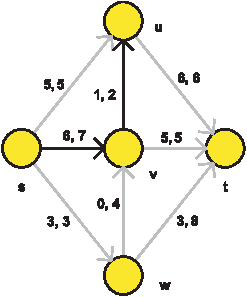
\includegraphics[width=45mm]{08/images/toky}
    \vspace{-10px}
  \end{center}
\end{wrapfigure}

\paragraph{Řez} je množina vrcholů, ve které je zdroj ale není spotřebič Minimální řez je řez s minimální kapacitou, který odděluje zdroj a spotřebič.

\textbf{Spočítá se Ford-Fulkensonem} - vezmu TRUE vrcholy, když už nemůžeme najít zlepšující se cestu. Sečtu toky hran, které mi znemožnili zlepšení (tzn. ty které jsou nasycené, i ty zpětné!). \textbf{Kapacita řezu} je \textbf{rovna} velikosti \textbf{maximálního toku}.

V příkladě na obrázku chceme najít minimální řez. O něm víme, že jeho vrcholy získáme pomocí značkovací metody Ford-Fulkensona. Ta nejdřív označí zdroj, pak označí vrchol $v$, protože jinam nemůže (všude je nasyceno). Následně označí vrchol $u$ a z něho dál již nelze jít (všude je opět nasyceno). Tím jsou určeny vrcholy řezu ($\{s,v,u\}$).

Kapacita min. řezu je určena jako součet toků hran, které zabránili zlepšení (a nevedou uvnitř řezu). Tzn. hrana 6/6, 5/5, 0,4 a 3/3. Toky hran které \uv{odchází} sečteme, a toky zpětných hran (které přichází) odečteme $\rightarrow 6 + 5 - 0 + 3 = 14$. Kapacita řezu je rovna 14, stejně tak jako hodnota maximálního toku.

Párování je množina hran, kde žádné dvě nemají společný vrchol. Nebo také rozdělení vrcholů na dvě skupiny kde uvnitř skupiny nejsou hrany. Používá se k přiřazování lidí k taskům. Jde převést na toky nebo Maďarským algoritmem.

Tokama lze řešit velké množství problémů:

\begin{itemize}[itemsep=0px]
\item transport zásob
\item zaokrouhlování v excelu
\item multiprocesorové rozvrhování
\end{itemize}

\subsection{Multi-komoditní toky}
Tok, kde teče víc komodit. Řeší se pomocí LP nebo ILP - nutné nadefinovat Kirchhoffův zákon pro každou komoditu. 